\chapter[Engenharia de Software]{Engenharia de Software}

\section[Requisitos de Software]{Requisitos de Software}
Os requisitos de software foram levantados e utilizados na hora do desenvolvimento para alcançar os objetivos elencados para o jogo. 

\begin{itemize}
	\item Ter um módulo para classificação de EDO
		\begin{itemize}
			\item Ter fase de classificação de ordem
			\item Ter fase de classificação de tipo
			\item Ter fase de classificação de linearidade
			\item Ter fase de classificação de homogeneidade
			\item Ter fase de classificação de separável
			\item Ter fase de classificação de exata
			\item Escolher 20 questões aleatórias do banco de equações
		\end{itemize}

	\item Ter um módulo para resolução de EDO de 1ª ordem
		\begin{itemize}
			\item Ter fase de resolução de EDO 1ª ordem homogênea
			\item Ter fase de resolução de EDO 1ª ordem não homogênea
			\item Ter fase de resolução de EDO 1ª ordem exata
			\item Ter fase de resolução de EDO 1ª ordem não exata
			\item Escolher 10 pares de equações aleatórias do banco de equações
		\end{itemize}

	\item Estar disponível para download no google play
	\item Sinalizar ao usuário fases concluídas
	\item Permitir envio de bugs e erros
		\begin{itemize}
			\item Notificar se o erro é por falta de internet
			\item Notificar se o erro é por problema do servidor
		\end{itemize}

	\item Permitir envio de sugestões e feedback
		\begin{itemize}
			\item Notificar se o erro é por falta de internet
			\item Notificar se o erro é por problema do servidor			
		\end{itemize}

	\item Ter um módulo de envio de estatísticas
		\begin{itemize}
			\item Identificar o aluno pela matrícula
			\item Enviar estatísticas de classificação
				\begin{itemize}
					\item armazenar fases concluídas
					\item armazenar quantidade de vezes que cada fase foi concluída
					\item armazenar 20 questoes presentes na tentativa
					\item armanezar tempo total gasto em cada conclusão
				\end{itemize}
			\item Enviar estatísticas de resolução
				\begin{itemize}
					\item armazenar fases concluídas
					\item armazenar quantidade de vezes que cada fase foi concluída
					\item armazenar 10 questoes presentes na tentativa
					\item armanezar tempo total gasto em cada conclusão
				\end{itemize}
			\item Sinalizar ao usuário quando a estatística for enviada
			\item Sinalizar ao usuário quando a estatística não for enviada
				\begin{itemize}
					\item Notificar se o erro é por falta de internet
					\item Notificar se o erro é por problema do servidor
				\end{itemize}
		\end{itemize}
\end{itemize}

\section[Banco de dados]{Banco de dados} 
Na pasta banco existe um arquivo chamado \textbf{seeds.txt} que é o arquivo com as equações diferenciais para alimentar o banco de dados da aplicação aprEnDO. O script \textbf{equações.js} lê o arquivo de seeds equação por equação, faz a requisição para o Wolfran Alpha utilizando os códigos da pasta wolfran\_api e requisita todos os pod disponíveis (pod são os arrays de informação disponibilizados). Após ter os pods são filtradas as informações desejadas e salvas em arquivos de informações localizadas na pasta \textbf{info}. Os pods apresentam as\textit{urls} das imagens de pergunta e das equações de resposta, quando existe resposta. Equações sem solução só podem ser utilizadas no primeiro módulo do jogo, o de classificação e não são incluídas no módulo de resolução. As imagens de perguntas baixadas são salvas na pasta \textbf{pergunta} e as imagens de respostas salvas na pasta \textbf{resposta}.

Com todas as informações desejadas de cada equação é possível utilizar o arquivo \textbf{estatisticas.js} que lê todos os arquivos de informação para contabilizar as informações da quantidade de equações diferenciais, quais tem resposta e quais não, quais são homogêneas, exatas, separáveis, linear, não linear, ordem1, ordem2, ordem3, ordem de 4 para cima são consideradas ordem superior, além de fazer a contagem total,também são indicados o número da equação. Essas informações são escritas num arquivo de controle para que possa ser lido pelo aplicativo aprEnDO e fazer a seleção das equações correta para renderizar, a depender do nível que a pessoa está jogando. O nome do arquivo de controle é \textbf{DADOS\_GERAIS.json}.


\section[Ambiente de desenvolvimento]{Ambiente de desenvolvimento}

O diagrama de classe foi modelado de modo a facilitar o desenvolvimento, pois deu uma guiada no que precisava ser feito e como as classes do jogo e os componentes se relacionam. 

\begin{figure}[H]
\centering
\caption{Diagrama de Classe do AprEnDO}
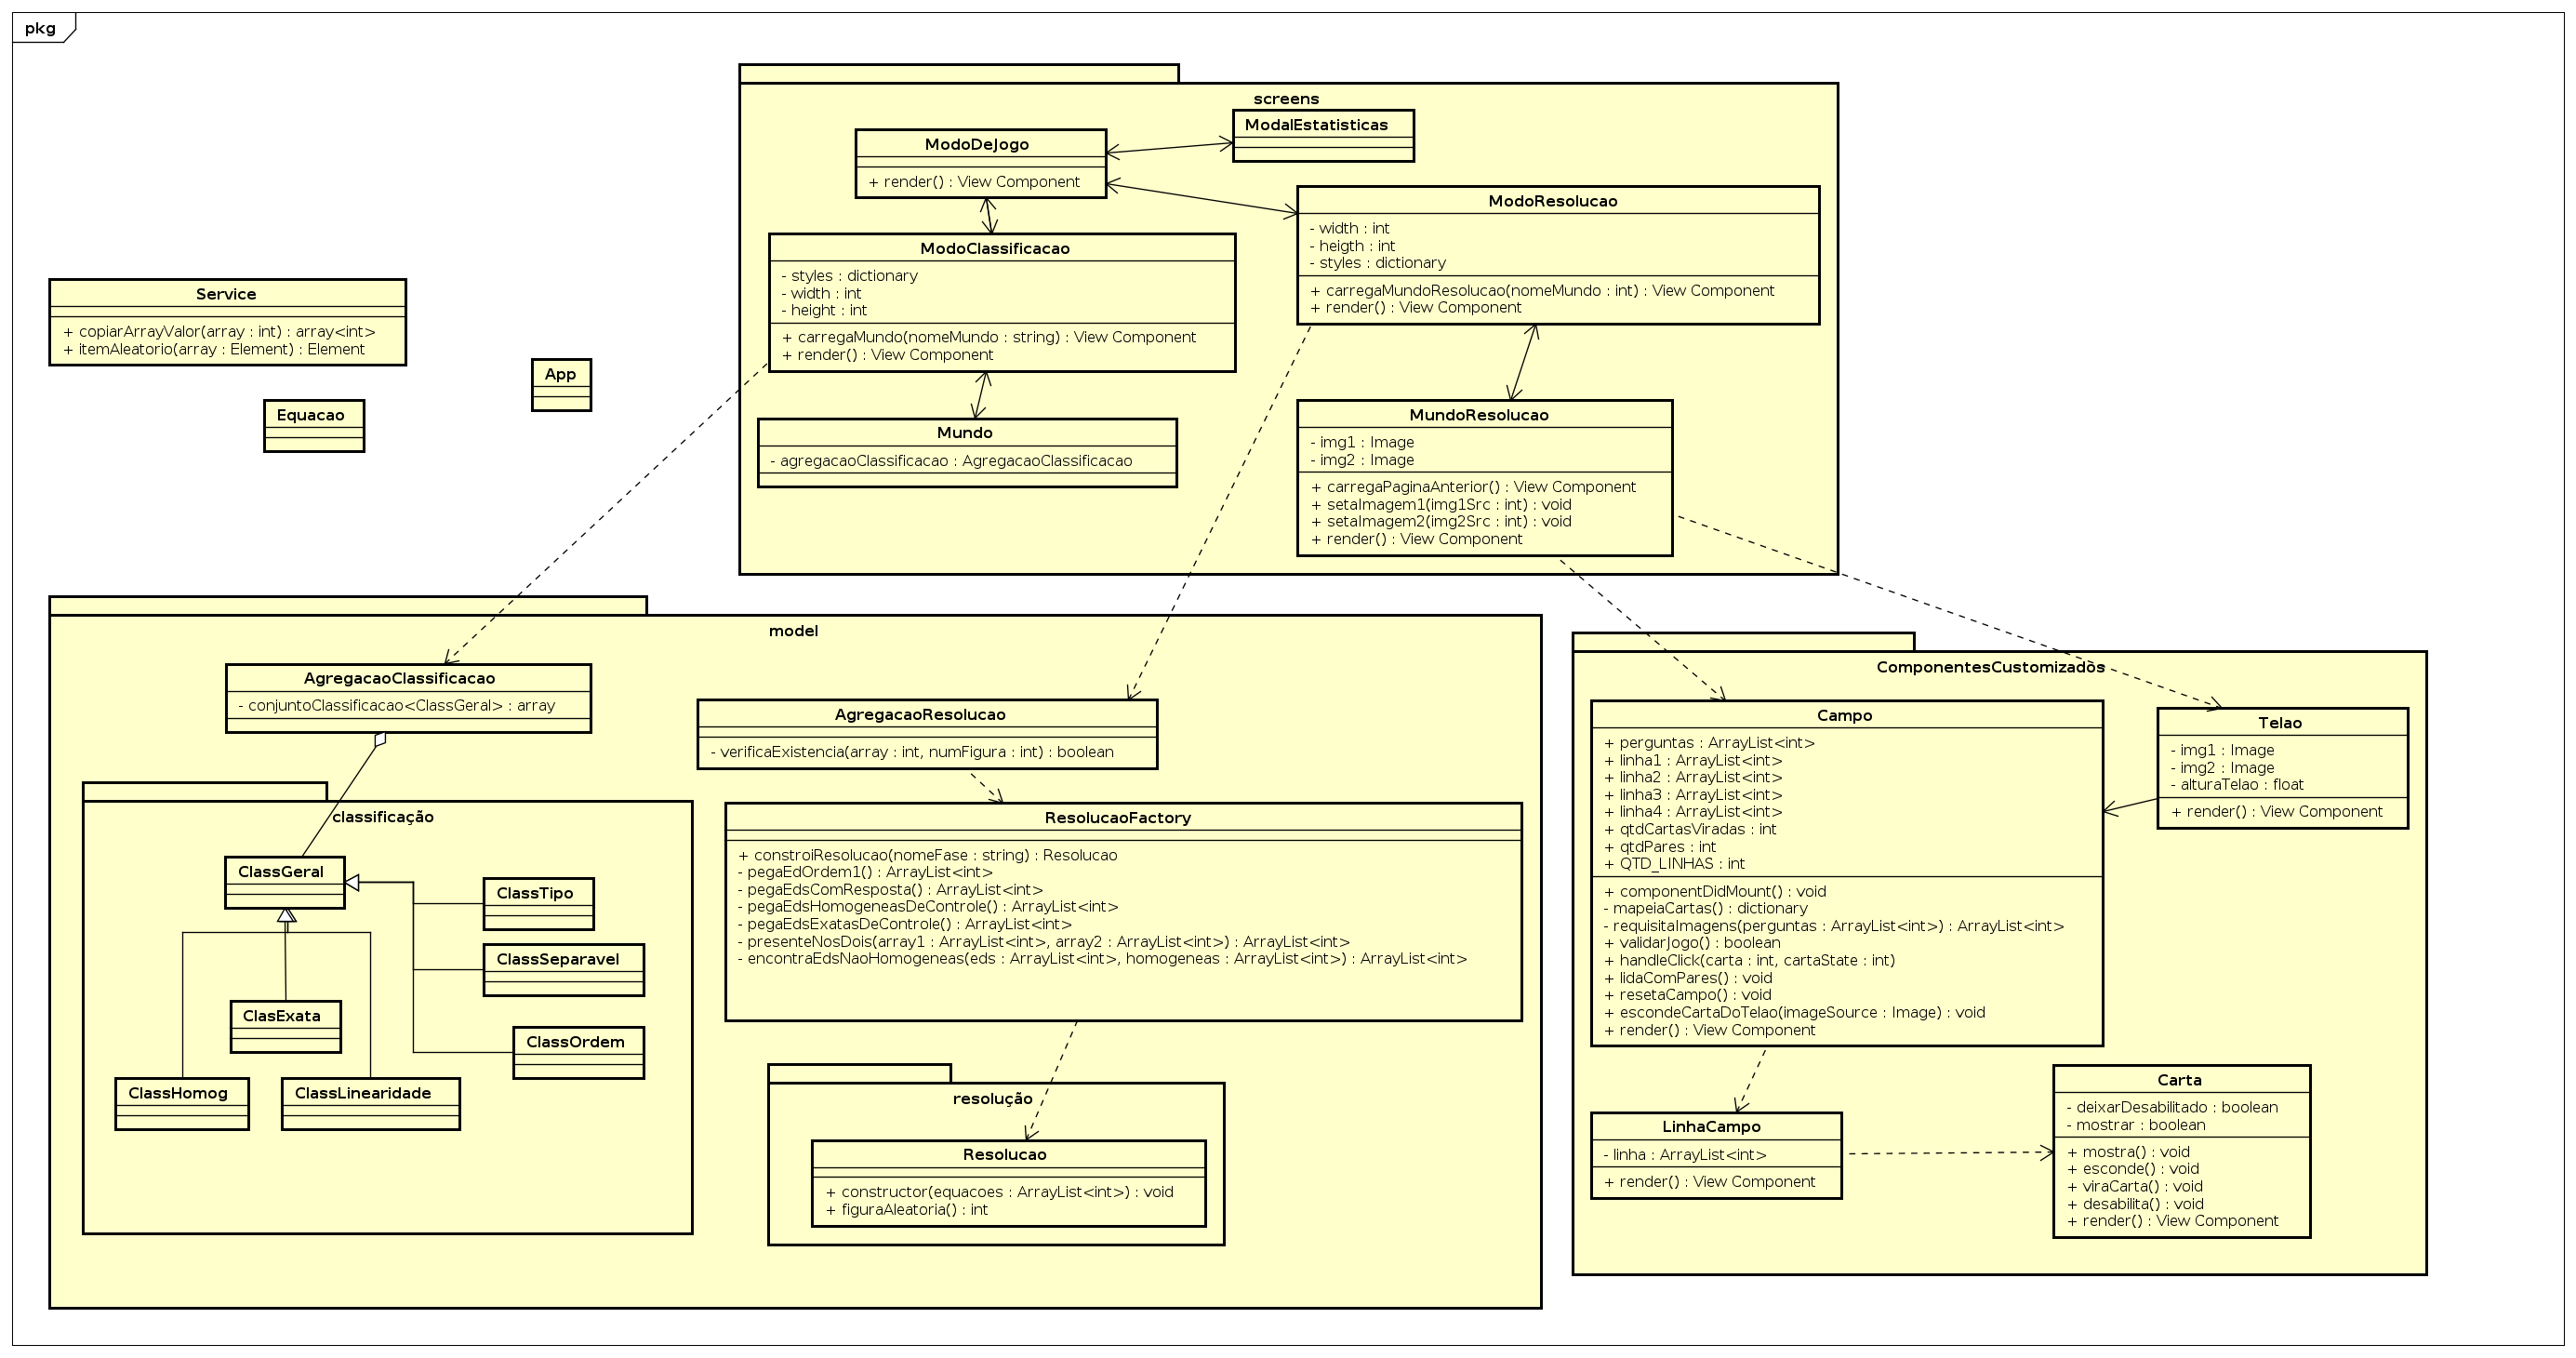
\includegraphics[scale=0.4]{figuras/diagramaClasse0_2.png}

\small{Fonte: do próprio autor}
\end{figure}


A linguagem de programação utilizada é o nodejs com o framework react native para gerar aplicação em código nativo android. Para baixar os pacotes e fazer o controle dos mesmos está sendo utilizado o nvm e o yarn.

O ambiente de desenvolvimento usa um emulador para simular a tela.

O WolfranAlpha será utilizado para fazer requisições de EDO's para serem utilizadas nas fases do jogo. Com uma chave de teste gratuita serão baixados os metad    ados em formato JSON através de uma API.
A API baixada do wolfran na linguagem javascript foi baixada no endereço \url{h    ttps://products.wolframalpha.com/api/libraries/javascript/}.
A chave gratuita permite 2000 requisições em um mês, com o código de série: 3GGQAT-98EG4KV6VL. A estratégia é baixar os metadados das requisições de EDO's com     equações e respostas, para comprimir e utilizar no jogo sem que a internet seja um requisito para jogar, porém para enviar dados ao servidor será necessário o acesso à internet.

\section[Empacotamento]{Empacotamento}
O jogo é empacotado para criar um arquivo .apk, e este que é instalado nos celulares. Para submeter o jogo ao Google Play para os jogadores poderem baixá-lo é necessário criar o .apk. O mesmo só é criado sempre que tem alguma nova atualização no jogo, seja no banco de equações ou manutenção corretiva ou evolutiva do jogo.

O empacotamento do jogo ocorre dentro da pasta do projeto react native. É utilizado o comando 'npm run android'.

\section[Servidor aprEnDO]{Servidor aprEnDO}
O servidor aprendo hospedado no heroku serve para receber estatísticas dos aplicativos enviados pelos alunos. Os alunos para enviar a estatística precisam informar o número da matrícula. As informações são enviadas em formato JSON e armazenadas em arquivos no servidor. 


\begin{comment}
////
A respeito do jogo, como colher dados? Os dados são colhidos quando o jogador está utilizando o jogo. Porém o dados são mantidos apenas no dispositivo. A pessoa pode enviar a estatística quando desejar, o professor solicitará o envio constante dos dados dos alunos.

Como enviar estatísticas? Haverá um botão responsável de enviar estatísticas, que podem ser enviadas para o servidor através do jogo em apenas um clique e uma confirmação do jogador. Assim que enviadas, as estatísticas armazenadas no celular se apagam para que no próximo envio não hajam informações repetidas.

Os dados colhidos e enviados são separados fase e módulos.

Por pergunta:\\
	- Qual é a pergunta alvo\\
	- Número das 4 EDs\\
	- Quantas tentativas foram necessárias para acertar a pergunta. **para saber se clicam aleatório ou escolhem antes de clicar **\\
	- Tempo gasto em cada pergunta  **para saber se a tela não ficou parada e o celular sem atenção**\\

	Algumas observações são: o clique pode demorar para acontecer ou acontecer muito rápido e as consequências podem ser acertar de primeira ou não acertar de primeira.\\
	Algumas inferências são: 
	cliques muito rápidos e não acertar de primeira == PODE significar chute aleatório\\
	cliques muito rápidos e acertar de primeira == pode ser um robô? alunos muito bem preparados?\\
	cliques devagar e não acertar de primeira == tá muito difícil? O celular está parado? \\
	cliques devagar e acertar de primeira == estava pensando? Estava resolvendo? O celular estava parado?\\

Por fase:\\
	- Quanto tempo durou cada fase (de 20 perguntas)\\

Dentro de cada módulo:\\
	- Quantas vezes clickou para jogar em uma fase(linear,exata,etc..) de classificação e saiu? (após 3 \\segundos)
	- Quantas vezes clickou para jogar em uma fase(homog, exata, etc) de resolução e saiu? (após 3 \\segundos)
	- Tempo total no módulo de classificação\\
	- Tempo total no módulo de resolução\\
	- Quantas vezes entrou e saiu de cada módulo (considerar que saiu é após 3 segundos).\\


Quantas vezes cada módulo foi clickado para jogar, e quantas ficaram sendo jogados mesmo.

Será avaliado dos mapas conceituais se houve evolução significativa entre os mapas conceituais dos alunos participantes em relação aos não participantes do jogo.
As estatísticas do jogo será para avaliar o desempenho dos alunos e qual a aceitação do jogo pelos participantes, para saber se é uma estratégia que pode ser levada adiante ou não.
\end{comment}